\documentclass{article} % For LaTeX2e
\usepackage{nips15submit_e,times}
\usepackage[colorlinks,linkcolor=red]{hyperref}
\usepackage{url}
\usepackage{amsmath}
\usepackage{graphicx}
\usepackage{float}
\usepackage{bm}
\usepackage{amssymb}
%\documentstyle[nips14submit_09,times,art10]{article} % For LaTeX 2.09


\title{CS499 Homework 7 (First Draft)}


\author{
	Intersteller\thanks{ Use footnote for providing further information
		about author (webpage, alternative address)---\emph{not} for acknowledging
		funding agencies.}
	Department of Computer Science
	Cranberry-Lemon University
	Pittsburgh, PA 15213
}

% The \author macro works with any number of authors. There are two commands
% used to separate the names and addresses of multiple authors: \And and \AND.
%
% Using \And between authors leaves it to \LaTeX{} to determine where to break
% the lines. Using \AND forces a linebreak at that point. So, if \LaTeX{}
% puts 3 of 4 authors names on the first line, and the last on the second
% line, try using \AND instead of \And before the third author name.

\newcommand{\fix}{\marginpar{FIX}}
\newcommand{\new}{\marginpar{NEW}}

%\nipsfinalcopy % Uncomment for camera-ready version

\begin{document}

	\maketitle
	\textbf{Exercise 7.1}\par
	\textbf{(1)}  Since e is in the minimum spanning tree, we split the minimum spanning tree into two components by deleting e. Let the vertices in the two components consist $S$ and $V\backslash S$ respectively. Since there is no circle in a tree, obviously e is the only edge which is good and cross this cut, which means no edge from X crosses this cut. \par
	\textbf{(2)}  Suppose e is not the minimum weight edge crossing this cut, assume there is an edge e' which has less weight and crosses this cut. e' can replace e and consists a spanning tree with less weight. This means e is not in the minimum spanning tree, which means e is not good, which contradicts the condition.\par
	\textbf{Exercies 7.4}
	\begin{figure}[H]
		\centering
		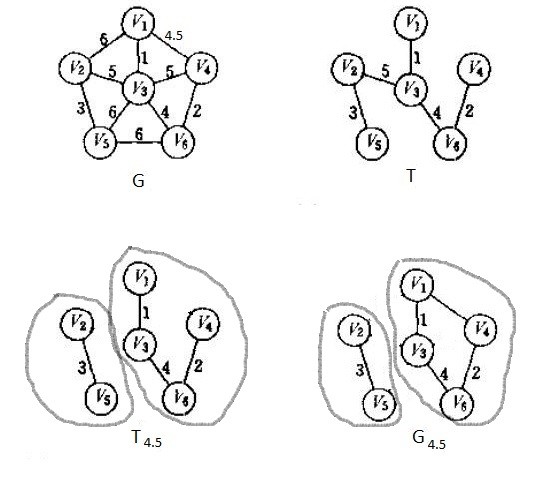
\includegraphics[scale=0.6]{P1.png}
		\caption{}
		\label{fig:1}
	\end{figure}

	\textbf{Exercies 7.5}
	Obviously, if two vertices are connected in $T_c$, they are connected in $G_c$, since $T_c$ is in $G_c$.\\
	Suppose u,v are connected in $G_c$, but not connected in $T_c$. Let two connected components in $T_c$ contain u and v respectively be A and B. Let e be an edge in $G_c$ that connect A and B. Using defination, $w(e)\leq c$. Since A and B are not connected in $T_c$, there must be an edge e' in T that connects A and B, and $w(e')>c$. So, e'>e. Obviously T which contains e' is not the minimum spanning tree, since e' can be replaced by e with less weight. This contradicts the condition. So, if two vertices are connected in $G_c$, they are connected in $T_c$.\par 
    
	\textbf{Question:}\par
	\textbf{1.}  In Exercise 7.11 \& 7.12, how can we compute the number of functions with a core of size $k$? $(1\leq k\leq n)$



\end{document}
	

